\begin{frame}[fragile]{Using UHD from Python (7/7)}

\footnotesize

\begin{itemize}
    \item \textbf{\textcolor{DarkBlue}{Step 7: Running the Python Receiver on X310}}
\end{itemize}

\hspace{2.8em}
\parbox{0.88\linewidth}{
\footnotesize
After replacing the device argument with the X310 IP address,
the remaining Python code and execution command remain unchanged.
}

\vspace{0.2cm}

\scriptsize
\begin{Verbatim}[xleftmargin=3.8em,breaklines,breaksymbolleft={},breaksymbolright={}]
python3 basic_rx_X310.py -f 100e6 -r 1e6 -d 5 -o rx_x310.npy -g 70
\end{Verbatim}

\vspace{0.25cm}
\begin{itemize}

    \begin{itemize}
        \item \scriptsize Only the USRP device argument changes.
        \item The UHD Python API remains identical for both devices.
        \item The same APIs can be used with B200/B210, X300/X310, N3xx,
              X410 and other supported USRPs.
    \end{itemize}
\end{itemize}
\vspace{0.3cm}

\begin{center}
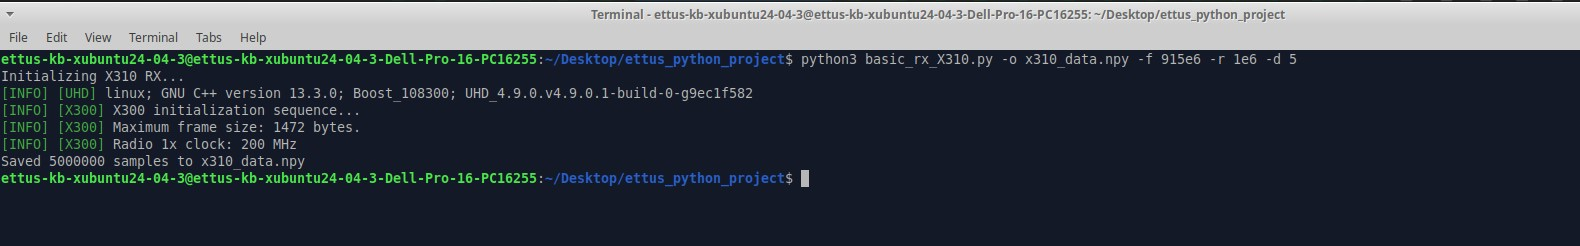
\includegraphics[width=0.90\linewidth,height=0.38\textheight,keepaspectratio]
{latex/jpg_png/image_python_api_X310_code_usage.jpg}
\end{center}

\end{frame}